\section*{The question, and the finding}

Genome-wide genetic correlation averages over a million variants. For a trait
whose heritability sits in one or two loci, that average is dominated by the
$\sim$999{,}900 variants doing nothing. The question here is whether bipred's
polygenic-overlap parameterisation recovers a relationship that \texttt{rg}
dilutes to noise.

Lipoprotein(a) is the case that makes it matter: essentially monogenic at
\emph{LPA}, a validated causal risk factor for coronary artery disease, and the
target of phase-3 lowering trials. If \texttt{rg} cannot see that relationship,
it is the wrong summary for a whole class of clinically important exposures.

It cannot. Fitted against CAD over 958{,}782 variants, Lp(a) has a genome-wide
\texttt{rg} of $+0.0712$, and cross-trait LD Score regression puts the same
quantity at $-0.0947$ (se $0.1238$) --- pointing the wrong way, and within one
standard error of zero either way. The same fit estimates 96 causal variants
for Lp(a) against 1{,}537 for CAD, 55 of them shared, with effects inside that
shared component correlating $+0.5170$.

\begin{figure}[H]
\centering
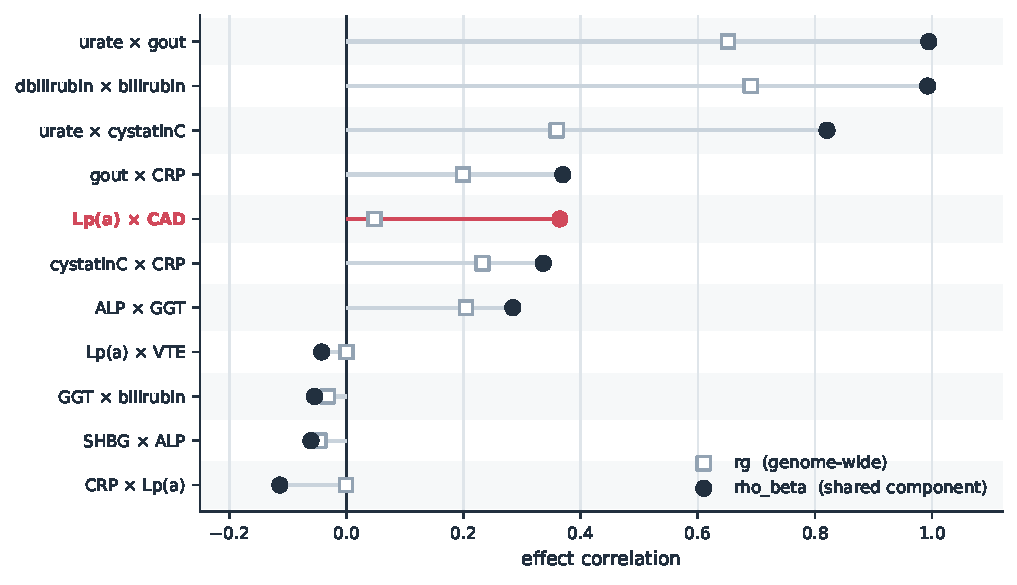
\includegraphics[width=\linewidth]{figures/rho-beta-vs-rg.pdf}
\caption{Pairs ordered by \texttt{rho\_beta}, with genome-wide \texttt{rg} on
the same row. The order is biological: same-biology and causal pairs at the
top, unrelated pairs at the bottom. \texttt{rho\_beta} exceeds \texttt{rg}
almost everywhere, because \texttt{rg} is attenuated by the variants that carry
no signal for either trait. What distinguishes Lp(a) $\times$ CAD is the size of
the gap. Compare gout $\times$ CRP two rows below it, which reaches
\texttt{rho\_beta} $+0.3083$ on an \texttt{rg} of $+0.1533$: a smaller
architecture correlation built on a genome-wide average twice as large. Lp(a)
$\times$ CAD reaches $+0.5170$ on an \texttt{rg} of $+0.0712$.}
\end{figure}

The two pairs at the top are there because their answers were known in advance:
direct against total bilirubin is two studies of the same biology, and urate
against gout has crystal deposition as the disease mechanism. Both land above
$+0.98$, which is what fixes the top of the scale. Three pairs sit below zero,
between $-0.11$ and $-0.03$: SHBG $\times$ ALP and CRP $\times$ Lp(a), chosen
because no shared biology was expected, and Lp(a) $\times$ VTE. A fourth
intended null, GGT $\times$ bilirubin, is not in the figure --- its uncapped
fit diverged, and \emph{The chi-square cap} explains why. Without both ends of
this scale, $+0.5170$ would be a number with nothing to compare it to.

Lp(a) $\times$ CAD ranks fourth of the ten admissible pairs. Above it are only
the two calibration anchors and urate $\times$ cystatinC, where shared renal
handling is expected. It is the highest-ranked pair that is neither the same
trait measured twice nor a mechanism acting on its own disease.

\begin{figure}[H]
\centering
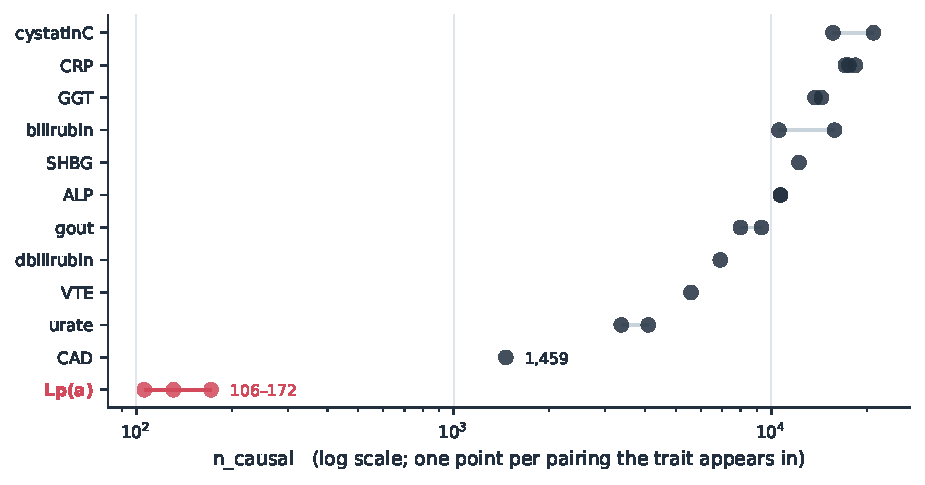
\includegraphics[width=\linewidth]{figures/polygenicity.pdf}
\caption{Estimated polygenicity per trait, one point per pairing the trait
appears in. Lp(a) is estimated at 90, 94 and 96 causal variants across three
independent pairings; every other trait here is in the thousands to tens of
thousands. Averaging $\sim$100 causal variants over $\sim$$10^6$ destroys the
signal in \texttt{rg}; the architecture summary does not average it away. The
open markers are the same fits with the chi-square cap applied to the joint
fit, and the arrows are what removing it does --- see \emph{The chi-square cap}.}
\end{figure}
